\documentclass{fizykalab}

% Variables
\def\pomvspace{\vspace{0.3em}}

% Ustawienia strony
\usepackage{lipsum}
\usepackage[margin=3cm]{geometry}
\usepackage{graphicx}
\usepackage{enumitem}
\usepackage{siunitx}
\usepackage{amsmath}
\usepackage{cancel}
\usepackage{makecell}
\usepackage{mathtools}
\setlist{leftmargin=15pt,labelindent=15pt}
\setlist[enumerate]{noitemsep,wide=0pt, leftmargin=*}

% Ustawienia stopki
\usepackage{lastpage}
\usepackage{fancyhdr}
\pagestyle{fancy}
\fancyhf{} % sets both header and footer to nothing
\renewcommand{\headrulewidth}{0pt}
\cfoot{\thepage\ z \pageref{LastPage}}

% Ustawienia do tabelki
\wydzial{IEiT}
\autorjeden{Robert Mesek}
\autordwa{}
\rok{II}
\grupa{8 - L}
\zespol{6}
\temat{Halotron}
\nrcwiczenia{43}
\datawykonania{10.10.2023}
\dataoddaniajeden{}
\zwrotdopoprawy{}
\dataoddaniadwa{}
\datazaliczenia{}

\begin{document}

\maketitle

\section*{Układ pomiarowy i oznaczenia}
 {\setlength{\parindent}{0pt}
  \begin{figure}[!ht]
	  \centering
	  \vspace{0pt}
	  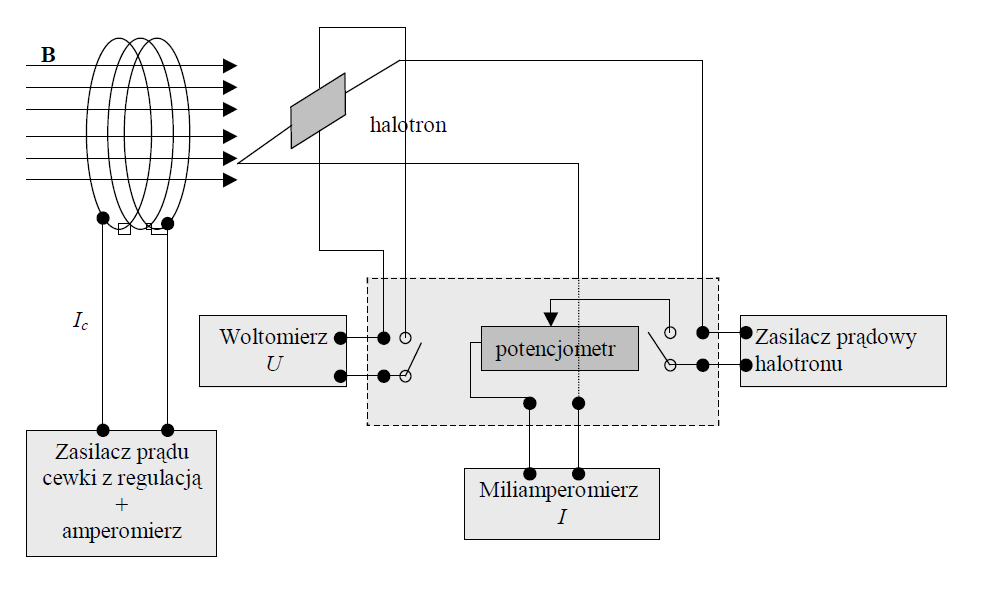
\includegraphics[width=1\linewidth]{images/uklad.png}
	  \caption{Schemat układu pomiarowego}
	  \label{fig:uklad-pomiarowy}
  \end{figure}

  \begin{minipage}[t]{1\textwidth}

	  \begin{enumerate}
		  \item [\textbf{Elementy układu pomiarowego (Rys.~\ref{fig:uklad-pomiarowy}):}]

		  \item Halotron połączony z: zasilaczem, woltomierzem, miliamperomierzem i potencjometrem do regulacji natężenia prądu.

		  \item Cewka podłączona do regulowanego zasilacza z amperomierzem.

	  \end{enumerate}

	  \paragraph{Specyfikacja urządzeń pomiarowych:}\mbox{}\newline
	  \textbf{Przy halotronie:}

	  \quad Rozdzielczość woltomierza \SI{0.1}{\milli\volt}

	  \quad Rozdzielczość miliamperomierza \SI{0.01}{\milli\ampere}

	  \textbf{Przy cewce:}

	  \quad Liczba zwojów cewki $N =$ \SI{40}{}

	  \quad Średnica cewki $r =$ \SI{110}{\milli\meter}

	  \quad Rozdzielczość amperomierza zasilacza \SI{0.2}{\ampere}

  \end{minipage}%
  \hspace*{\fill}
 }


\newpage

\section*{Ćwiczenie ,,43'': Halotron}
{\setlength{\parindent}{0pt}
\paragraph{Cel ćwiczenia:}
Cechowanie halotronu przy użyciu pola magnetycznego o znanej indukcji. Wykorzystanie halotronu do pomiaru przestrzennego rozkładu pola cewki kołowej i magnesu ferrytowego.
\newline

\par
Napięcie Halla to różnica potencjałów powstająca w przewodniku z prądem umieszczonym w polu magnetycznym. Na elektrony w halotronie działa siła Lorentza $\boldsymbol{F} = q\boldsymbol{v}\times\boldsymbol{B}$ gdzie $q$ oznacza ładunek elektronu, $\boldsymbol{v}$ jest wektorem średniej prędkości ruchu elektronu, zaś $\boldsymbol{B}$ wektorem indukcji magnetycznej.

Dla napięcia Halla $U_H$ występuje pole elektryczne $E_H = \frac{U_H}{d}$ gdzie $d$ to szerokość warstwy przewodzącej. Na elektrony działa więc siła $F_E = q \cdot E_H$. Obie te siły działają w przeciwnych kierunkach i w stanie równowagi otrzymujemy:
\begin{equation}
	U_H = vBd
	\tag{1}
\end{equation}
Gęstość prądu wyrażamy $j = \frac{I}{dh}$, a przyjmując $n$ jako koncentrację nośników, czyli liczbę nośników prądu w jednostce objętości,
\begin{equation}
	j=vnq
	\tag{2}
\end{equation}
Łącząc (1) i (2) otrzymujemy:
\begin{equation}
	U_H = \frac{1}{nqh}IB
	\tag{3}
\end{equation}
Współczynnik proporcjonalności $c = \frac{1}{ngh}$ to stała halotronu.

W efekcie oporu warstwy półprzewodnika zastosowanego do budowy halotronu, powstaje dodatkowe napięcie $U_R$ proporcjonalne do prądu halotronu. Ostatecznie mierzone napięcie wynosi:
\begin{equation}
	U = U_H + U_R = cIB + RI
	\tag{4}
\end{equation}

\par
Natężenie pola magnetycznego na osi cewki kołowej liczymy z prawa Biota-Savarta:
\begin{equation}
	B_0 = \frac{\mu_0 N I_S}{2R}
	\tag{5}
\end{equation}

Wykonując pomiary na osi solenoidu w odległości $z$ od jego środka korzystamy ze wzoru na indukcję magnetyczną:
\begin{equation}
	B(z) = \frac{B_0}{\left( 1 + \frac{z^2}{R^2} \right)^\frac{3}{2}}
	\tag{6}
\end{equation}

\mbox{}\newline\newline
\begin{figure}[!ht]
	\centering
	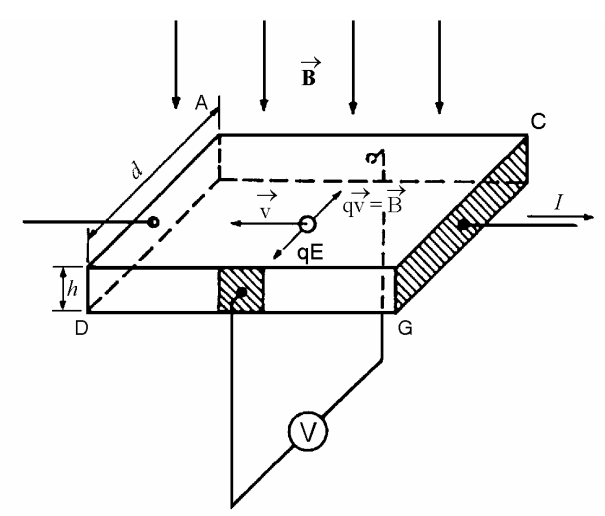
\includegraphics[width=0.4\linewidth]{images/halotron.png}
	\caption{Schemat halotronu}
	\label{fig:halotron}
\end{figure}


\newpage

\section*{Cechowanie halotronu}
{\setlength{\parindent}{0pt}
\subsection*{Wykonanie ćwiczenia}
\par
1. Korzystamy z obwodu zgodnego ze schematem (Rys.~\ref{fig:uklad-pomiarowy}).

2. Ustawiamy halotron w środku cewki:

\hspace*{1em}
\begin{minipage}{1\textwidth}
	a) przesuwając halotron w kierunku poziomym znaleźć położenie odpowiadające
	\\ maksymalnej wartości $U$

	b) przesuwając halotron w kierunku pionowym znaleźć położenie odpowiadające
	\\ minimalnej wartości $U$
\end{minipage}

3. Po uruchomieniu cewki wykonujemy pomiary dla trzech wartości prądu halotronu:

\hspace*{1em}
\begin{minipage}{1\textwidth}
	\quad \SI{5.0}{\milli\ampere}, \SI{7.5}{\milli\ampere}, \SI{10.0}{\milli\ampere}
\end{minipage}
\hspace*{1em}
\begin{minipage}{1\textwidth}
	oraz dla wartości prądu cewki od:

	\quad \SI{0}{} do \SI{10}{\ampere} ze skokiem \SI{1}{\ampere}
\end{minipage}


\subsection*{Wyniki pomiarów}
\par
\begin{table}[!ht]
	\centering
	\begin{tabular}{|c|ccccccccccc|}
		\hline
		Prąd cewki {[}\SI{}{\ampere}{]}           & \multicolumn{1}{l|}{0}                                        & \multicolumn{1}{l|}{1}   & \multicolumn{1}{l|}{2}   & \multicolumn{1}{l|}{3}    & \multicolumn{1}{l|}{4}    & \multicolumn{1}{l|}{5}    & \multicolumn{1}{l|}{6}    & \multicolumn{1}{l|}{7}    & \multicolumn{1}{l|}{8}    & \multicolumn{1}{l|}{9}    & 10   \\ \hline
		Prąd halotronu {[}\SI{}{\milli\ampere}{]} & \multicolumn{11}{c|}{Napięcie Halla {[}\SI{}{\milli\volt}{]}}                                                                                                                                                                                                                                                                  \\ \hline
		5.00                                      & \multicolumn{1}{l|}{4.2}                                      & \multicolumn{1}{l|}{4.6} & \multicolumn{1}{l|}{4.9} & \multicolumn{1}{l|}{5.3}  & \multicolumn{1}{l|}{5.6}  & \multicolumn{1}{l|}{6.0}  & \multicolumn{1}{l|}{6.4}  & \multicolumn{1}{l|}{6.7}  & \multicolumn{1}{l|}{7.1}  & \multicolumn{1}{l|}{7.4}  & 7.8  \\ \hline
		7.50                                      & \multicolumn{1}{l|}{6.3}                                      & \multicolumn{1}{l|}{6.8} & \multicolumn{1}{l|}{7.3} & \multicolumn{1}{l|}{7.8}  & \multicolumn{1}{l|}{8.4}  & \multicolumn{1}{l|}{8.9}  & \multicolumn{1}{l|}{9.5}  & \multicolumn{1}{l|}{10.0} & \multicolumn{1}{l|}{10.5} & \multicolumn{1}{l|}{11.1} & 11.6 \\ \hline
		10.00                                     & \multicolumn{1}{l|}{8.2}                                      & \multicolumn{1}{l|}{8.8} & \multicolumn{1}{l|}{9.4} & \multicolumn{1}{l|}{10.2} & \multicolumn{1}{l|}{10.9} & \multicolumn{1}{l|}{11.6} & \multicolumn{1}{l|}{12.3} & \multicolumn{1}{l|}{13.0} & \multicolumn{1}{l|}{13.7} & \multicolumn{1}{l|}{14.4} & 15.1 \\ \hline
	\end{tabular}
	\caption*{Tabela 1}
\end{table}

\subsection*{Opracowanie wyników}
\subsection*{Wykres i zależność liniowa z pomocą programu Excel}
\par
\begin{figure}[H]
	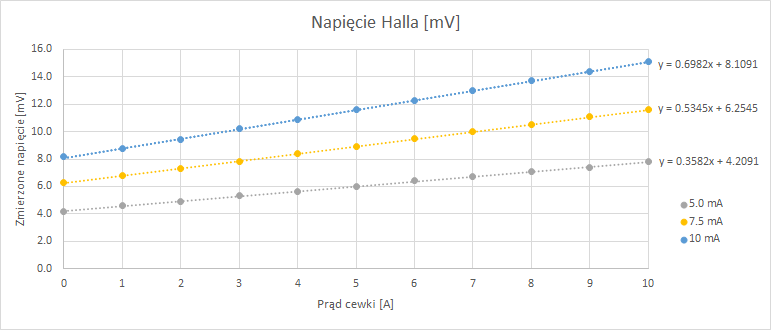
\includegraphics[width=1\linewidth]{images/wykres1.png}
	\centering
\end{figure}

\newpage

\paragraph{Obliczanie zależności liniowej}\mbox{}\newline
Z otrzymanej zależności liniowej $ax + b = I_c(cB) + RI_H \ (=U_h(I_c)\ )$ oraz wzoru 4 wyznaczymy zależności $c$ i $R$:
\begin{align*}
	R & = \frac{b}{I_H}
	\\
	c & = \frac{a \cdot 2r}{I_H \mu_0 N}
	\tag{7}
\end{align*}
Wykorzystamy otrzymane dane do wycechowania halotronu:
\begin{table}[H]
	\centering
	\begin{tabular}{|c|c|c|}
		\hline
		\rule{0pt}{1em}$I_H [\SI{}{\milli\ampere}]$ & $R [\SI{}{\ohm}]$ & $c [\frac{\SI{}{\ohm}}{\SI{}{\tesla}}]$ \\ \hline
		5.0                                         & 0.84              & 179.17                                  \\ \hline
		7.5                                         & 0.83              & 178.24                                  \\ \hline
		10.0                                        & 0.81              & 174.62                                  \\ \hline
	\end{tabular}
	\caption*{Tabela 2: Opór halotronu i stała halotronu}
\end{table}

\subsection*{Wartości średnie i niepewności}
\par
\[ \overline{R_H} = 0.83 \ [\SI{}{\ohm}] \quad\quad u(R_H) = 0.09 \ [\SI{}{\ohm}] \]
\[ \overline{c_H} = 177.34 \ \left[\frac{\SI{}{\ohm}}{\SI{}{\tesla}}\right] \quad\quad u(c_H) = 2.75 \ \left[\frac{\SI{}{\ohm}}{\SI{}{\tesla}}\right] \]

\subsection*{Ostateczny wynik}
\par
\[ R_H = 0.83 \pm 0.09 \ [\SI{}{\ohm}] \]
\[ c_H = 177.34 \pm 2.75 \ \left[\frac{\SI{}{\ohm}}{\SI{}{\tesla}}\right] \]

\subsection*{Wnioski}
\par
Napięcia Halla zachowuje się zgodnie z przewidywaniami.
Rośnie liniowo wraz ze wzrostem pola magnetycznego.
Znając to oraz prąd przepływający przez cewkę mogliśmy na ich podstawie wyznaczyć stała halotronu $c$ i opór halotronu $R$.


\newpage


\section*{Pomiar rozkładu pola magnetycznego wzdłuż osi cewki}
{\setlength{\parindent}{0pt}
\subsection*{Wykonanie ćwiczenia}
\par
1. Ustawiamy prąd halotronu oraz prąd cewki na wartości maksymalne.

2. Zaczynając od środka cewki przesuwamy halotron co 0.5cm i odczytujemy napięcie Halla.

\subsection*{Wyniki pomiarów}
\par
\begin{table}[H]
	\centering
	\begin{tabular}{|c|c|}
		\hline
		$x [\SI{}{\centi\meter}]$ & $U [\SI{}{\milli\volt}]$ \\ \hline
		0                         & 15.1                     \\ \hline
		0.5                       & 15.0                     \\ \hline
		1.0                       & 14.8                     \\ \hline
		1.5                       & 14.5                     \\ \hline
		2.0                       & 14.0                     \\ \hline
		2.5                       & 13.5                     \\ \hline
		3.0                       & 12.9                     \\ \hline
		3.5                       & 12.4                     \\ \hline
		4.0                       & 11.9                     \\ \hline
		4.5                       & 11.4                     \\ \hline
		5.0                       & 11                       \\ \hline
		5.5                       & 10.7                     \\ \hline
		6.0                       & 10.3                     \\ \hline
		6.5                       & 10.1                     \\ \hline
		7.0                       & 9.8                      \\ \hline
		7.5                       & 9.6                      \\ \hline
		8.0                       & 9.4                      \\ \hline
		8.5                       & 9.3                      \\ \hline
		9.0                       & 9.1                      \\ \hline
		9.5                       & 9.0                      \\ \hline
		10.0                      & 8.9                      \\ \hline
	\end{tabular}
	\caption*{Tabela 3: Rozkład pola magnetycznego wzdłuż osi cewki}
\end{table}

\subsection*{Obliczenia}
Korzystając z $c_H$ i $R_H$ otrzymanych podczas cechowania halotronu obliczamy wartość pola magnetycznego $B$ dla mierzonych odległości:
\begin{gather*}
	U = cIB + RI
	\\
	B = \frac{U}{cI} - \frac{R}{c}
	\tag{8}
\end{gather*}

\newpage

Wykorzystując wzór (6) uzupełnimy tabelę 3 o teoretyczne wartości wynikające z zależności:
\begin{gather*}
	B_0 = \frac{\mu_0 N I_S}{2R}
	\\
	B(z) = \frac{B_0}{\left( 1 + \frac{z^2}{R^2} \right)^\frac{3}{2}}
\end{gather*}
Dla $R = 0.055 \ [\SI{}{\meter}]$, $N = 70$ i $I_S = 10 \ [\SI{}{\ampere}]$:
\[ B_0 = 8.00 \ [\SI{}{\milli\tesla}] \]

\subsection*{Niepewności pomiaru}
\par
Niepewność pomiaru typu B napięcia halotronu $u(U_H)$ wynosi $\frac{0.1}{\sqrt{3}} \ \SI{}{\milli\volt}$.

Niepewności pomiaru typu B natężenia prądu halotronu $u(I_H)$ przyjmiemy za $\SI{0.01}{\milli\ampere}$ wynikające z dokładności amperomierza i potencjometru.

\mbox{}\newline
Obliczmy niepewności pomiarowe korzystając ze wzoru (8) i wpiszemy je do tabeli:
\begin{align*}
	u(B) & = \sqrt{\left( \frac{\partial B}{\partial U} \cdot u(U) \right)^2 + \left( \frac{\partial B}{\partial c} \cdot u(c) \right)^2 + \left( \frac{\partial B}{\partial I} \cdot u(I) \right)^2 + \left( \frac{\partial B}{\partial R} \cdot u(R) \right)^2}
	\\
	u(B) & = \sqrt{\left( \frac{u(U)}{cI} \right)^2 + \left( \left( \frac{R}{c^2} - \frac{U}{c^2I} \right) \cdot u(c) \right)^2 + \left( \frac{U}{cI^2} \cdot u(I) \right)^2 + \left( \frac{1}{c} \cdot u(R) \right)^2}
	\\
	u(B) & = \frac{1}{c} \cdot \sqrt{\left( \frac{u(U)}{I} \right)^2 + \left( \left( \frac{R}{c} - \frac{U}{cI} \right) \cdot u(c) \right)^2 + \left( \frac{U}{I^2} \cdot u(I) \right)^2 + \left( u(R) \right)^2}
	\tag{9}
\end{align*}

\subsection*{Wykres wyników na podstawie tabeli 4}
\begin{figure}[H]
	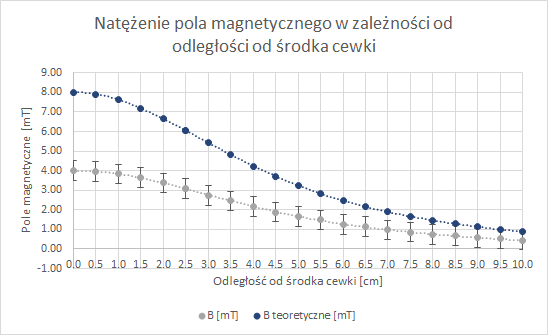
\includegraphics[width=0.8\linewidth]{images/wykres2.png}
	\centering
\end{figure}

\subsection*{Wyniki obliczeń}
\begin{table}[H]
	\centering
	\begin{tabular}{|c|c|c|c|}
		\hline
		$x [\SI{}{\centi\meter}]$ & $U [\SI{}{\milli\volt}]$ & $B [\SI{}{\milli\tesla}]$ & $B$ teoretyczne $[\SI{}{\milli\tesla}]$ \\ \hline
		$0.0$                     & $15.1$                   & $4.00 \pm 0.52$           & $8.00$                                  \\ \hline
		$0.5$                     & $15.0$                   & $3.95 \pm 0.52$           & $7.90$                                  \\ \hline
		$1.0$                     & $14.8$                   & $3.83 \pm 0.52$           & $7.62$                                  \\ \hline
		$1.5$                     & $14.5$                   & $3.66 \pm 0.52$           & $7.18$                                  \\ \hline
		$2.0$                     & $14.0$                   & $3.37 \pm 0.52$           & $6.64$                                  \\ \hline
		$2.5$                     & $13.5$                   & $3.09 \pm 0.52$           & $6.04$                                  \\ \hline
		$3.0$                     & $12.9$                   & $2.74 \pm 0.52$           & $5.41$                                  \\ \hline
		$3.5$                     & $12.4$                   & $2.46 \pm 0.52$           & $4.80$                                  \\ \hline
		$4.0$                     & $11.9$                   & $2.17 \pm 0.52$           & $4.23$                                  \\ \hline
		$4.5$                     & $11.4$                   & $1.88 \pm 0.52$           & $3.71$                                  \\ \hline
		$5.0$                     & $11.0$                   & $1.66 \pm 0.52$           & $3.24$                                  \\ \hline
		$5.5$                     & $10.7$                   & $1.48 \pm 0.52$           & $2.83$                                  \\ \hline
		$6.0$                     & $10.3$                   & $1.25 \pm 0.52$           & $2.47$                                  \\ \hline
		$6.5$                     & $10.1$                   & $1.14 \pm 0.52$           & $2.16$                                  \\ \hline
		$7.0$                     & $9.8$                    & $0.97 \pm 0.52$           & $1.89$                                  \\ \hline
		$7.5$                     & $9.6$                    & $0.85 \pm 0.52$           & $1.65$                                  \\ \hline
		$8.0$                     & $9.4$                    & $0.74 \pm 0.52$           & $1.45$                                  \\ \hline
		$8.5$                     & $9.3$                    & $0.68 \pm 0.52$           & $1.28$                                  \\ \hline
		$9.0$                     & $9.1$                    & $0.57 \pm 0.52$           & $1.13$                                  \\ \hline
		$9.5$                     & $9.0$                    & $0.51 \pm 0.52$           & $1.01$                                  \\ \hline
		$10.0$                    & $8.9$                    & $0.45 \pm 0.52$           & $0.90$                                  \\ \hline
	\end{tabular}
	\caption*{Tabela 4: Pomiar rozkładu pola magnetycznego}
\end{table}

\subsection*{Wnioski}
\par
Otrzymane wyniki pola magnetycznego w przypadku cewki znacznie odbiegają od wartości teoretycznych. 
Mimo tego krzywa wartości obliczonych i wartości teoretycznych ma bardzo zbliżony kształt, jej wartości są przeskalowane (są dwukrotnie mniejsze).

Może to wynikać z braku kalibracji lub wady użytego halotronu.

\mbox{}\newline
Dodatkowo dla wartości już w odległości powyżej $\SI{5}{\centi\meter}$ błąd pomiarowy zaczyna zbytnio zniekształcać nasze wyniki, aby moglibyśmy być pewni ich poprawności.

\newpage

\section*{Pomiar indukcji pola magnetycznego dla magnesu stałego}
{\setlength{\parindent}{0pt}
\subsection*{Wykonanie ćwiczenia}
\par
1. Wyłączamy prąd cewki i mocujemy magnes stały w osi halotronu.

2. Zaczynając od 1cm odsuwamy magnes i odczytujemy napięcie Halla.

\subsection*{Wyniki pomiarów}
\par
\begin{table}[H]
	\centering
	\begin{tabular}{|c|c|}
		\hline
		$x [\SI{}{\centi\meter}]$ & $U [\SI{}{\milli\volt}]$ \\ \hline
		1.0                       & $+18.0$                  \\ \hline
		1.5                       & $+7.7$                   \\ \hline
		2.0                       & $+1.3$                   \\ \hline
		2.5                       & $-1.9$                   \\ \hline
		3.0                       & $-3.9$                   \\ \hline
		3.5                       & $-5.1$                   \\ \hline
		4.0                       & $-5.9$                   \\ \hline
		4.5                       & $-6.5$                   \\ \hline
		5.0                       & $-6.9$                   \\ \hline
		5.5                       & $-7.2$                   \\ \hline
		6.0                       & $-7.4$                   \\ \hline
		6.5                       & $-7.5$                   \\ \hline
		7.0                       & $-7.6$                   \\ \hline
		7.5                       & $-7.7$                   \\ \hline
		8.0                       & $-7.8$                   \\ \hline
		8.5                       & $-7.8$                   \\ \hline
		9.0                       & $-7.9$                   \\ \hline
		9.5                       & $-7.9$                   \\ \hline
		10.0                      & $-8.0$                   \\ \hline
		$\infty$                  & $-8.2$                   \\ \hline
	\end{tabular}
	\caption*{Tabela 5: Napięcie Halla w zależności od odległości od osi cewki, dla $\infty$ magnes był zdjęty z prowadnicy}
\end{table}

\subsection*{Obliczenia}
Do obliczenia pola magnetycznego wykorzystamy wzór (8) analogicznie z poprzednim doświadczeniem.

\mbox{}\newline
Zauważamy już, że dane wyglądają nietypowo, woltomierz wskazuje napięcie z ujemnym znakiem, gdy oddalamy magnes. Przy całkowitym odsunięciu magnesu woltomierz także wskazuje wartość ujemną napięcia.

\newpage

\subsection*{Wykres oraz wyniki obliczeń}
\begin{table}[H]
	\centering
	\begin{tabular}{|c|c|c|}
		\hline
		$x [\SI{}{\centi\meter}]$ & $U [\SI{}{\milli\volt}]$ & $B [\SI{}{\milli\tesla}]$ \\ \hline
		$1.00$                    & $+18.00$                 & $+5.66$                   \\ \hline
		$1.50$                    & $+7.70$                  & -$0.23$                   \\ \hline
		$2.00$                    & $+1.30$                  & -$3.90$                   \\ \hline
		$2.50$                    & -$1.90$                  & -$5.73$                   \\ \hline
		$3.00$                    & -$3.90$                  & -$6.88$                   \\ \hline
		$3.50$                    & -$5.10$                  & -$7.56$                   \\ \hline
		$4.00$                    & -$5.90$                  & -$8.02$                   \\ \hline
		$4.50$                    & -$6.50$                  & -$8.37$                   \\ \hline
		$5.00$                    & -$6.90$                  & -$8.60$                   \\ \hline
		$5.50$                    & -$7.20$                  & -$8.77$                   \\ \hline
		$6.00$                    & -$7.40$                  & -$8.88$                   \\ \hline
		$6.50$                    & -$7.50$                  & -$8.94$                   \\ \hline
		$7.00$                    & -$7.60$                  & -$9.00$                   \\ \hline
		$7.50$                    & -$7.70$                  & -$9.05$                   \\ \hline
		$8.00$                    & -$7.80$                  & -$9.11$                   \\ \hline
		$8.50$                    & -$7.80$                  & -$9.11$                   \\ \hline
		$9.00$                    & -$7.90$                  & -$9.17$                   \\ \hline
		$9.50$                    & -$7.90$                  & -$9.17$                   \\ \hline
		$10.00$                   & -$8.00$                  & -$9.23$                   \\ \hline
		$\infty$                  & $-8.2$                   & -$9.34$                   \\ \hline
	\end{tabular}
	\caption*{Tabela 6: Obliczenia pola magnetycznego w zależności odległości magnesu od halotronu}
\end{table}

\begin{figure}[H]
	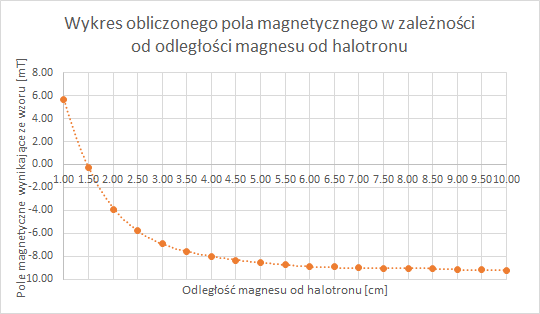
\includegraphics[width=0.6\linewidth]{images/wykres3.png}
	\centering
\end{figure}

\subsection*{Wnioski}
\par
W tym przypadku wada lub brak kalibracji halotronu jest bardzo widoczny, ponieważ korzystając z wyprowadzonego wzoru otrzymujemy ujemne wartości pola magnetycznego. 
Dodatkowo przy całkowitym odsunięciu magnesu, nadal występuje napięcie Halla o ujemnej wartości. 
Aby dowiedzieć co nie udało się z naszymi obliczeniami moglibyśmy sprawdzić natężenie pola magnetycznego innym już skalibrowanym miernikiem oraz określić bazowe pole magnetyczne przy naszym stanowisku mogące wynikać z czynników zewnętrznych.

Mimo tego pole magnetyczne maleje wraz ze zwiększaniem odległości magnesu od halotronu, a także krzywa ma kształt podobny do oczekiwanego.

\newpage
\begin{figure}[H]
	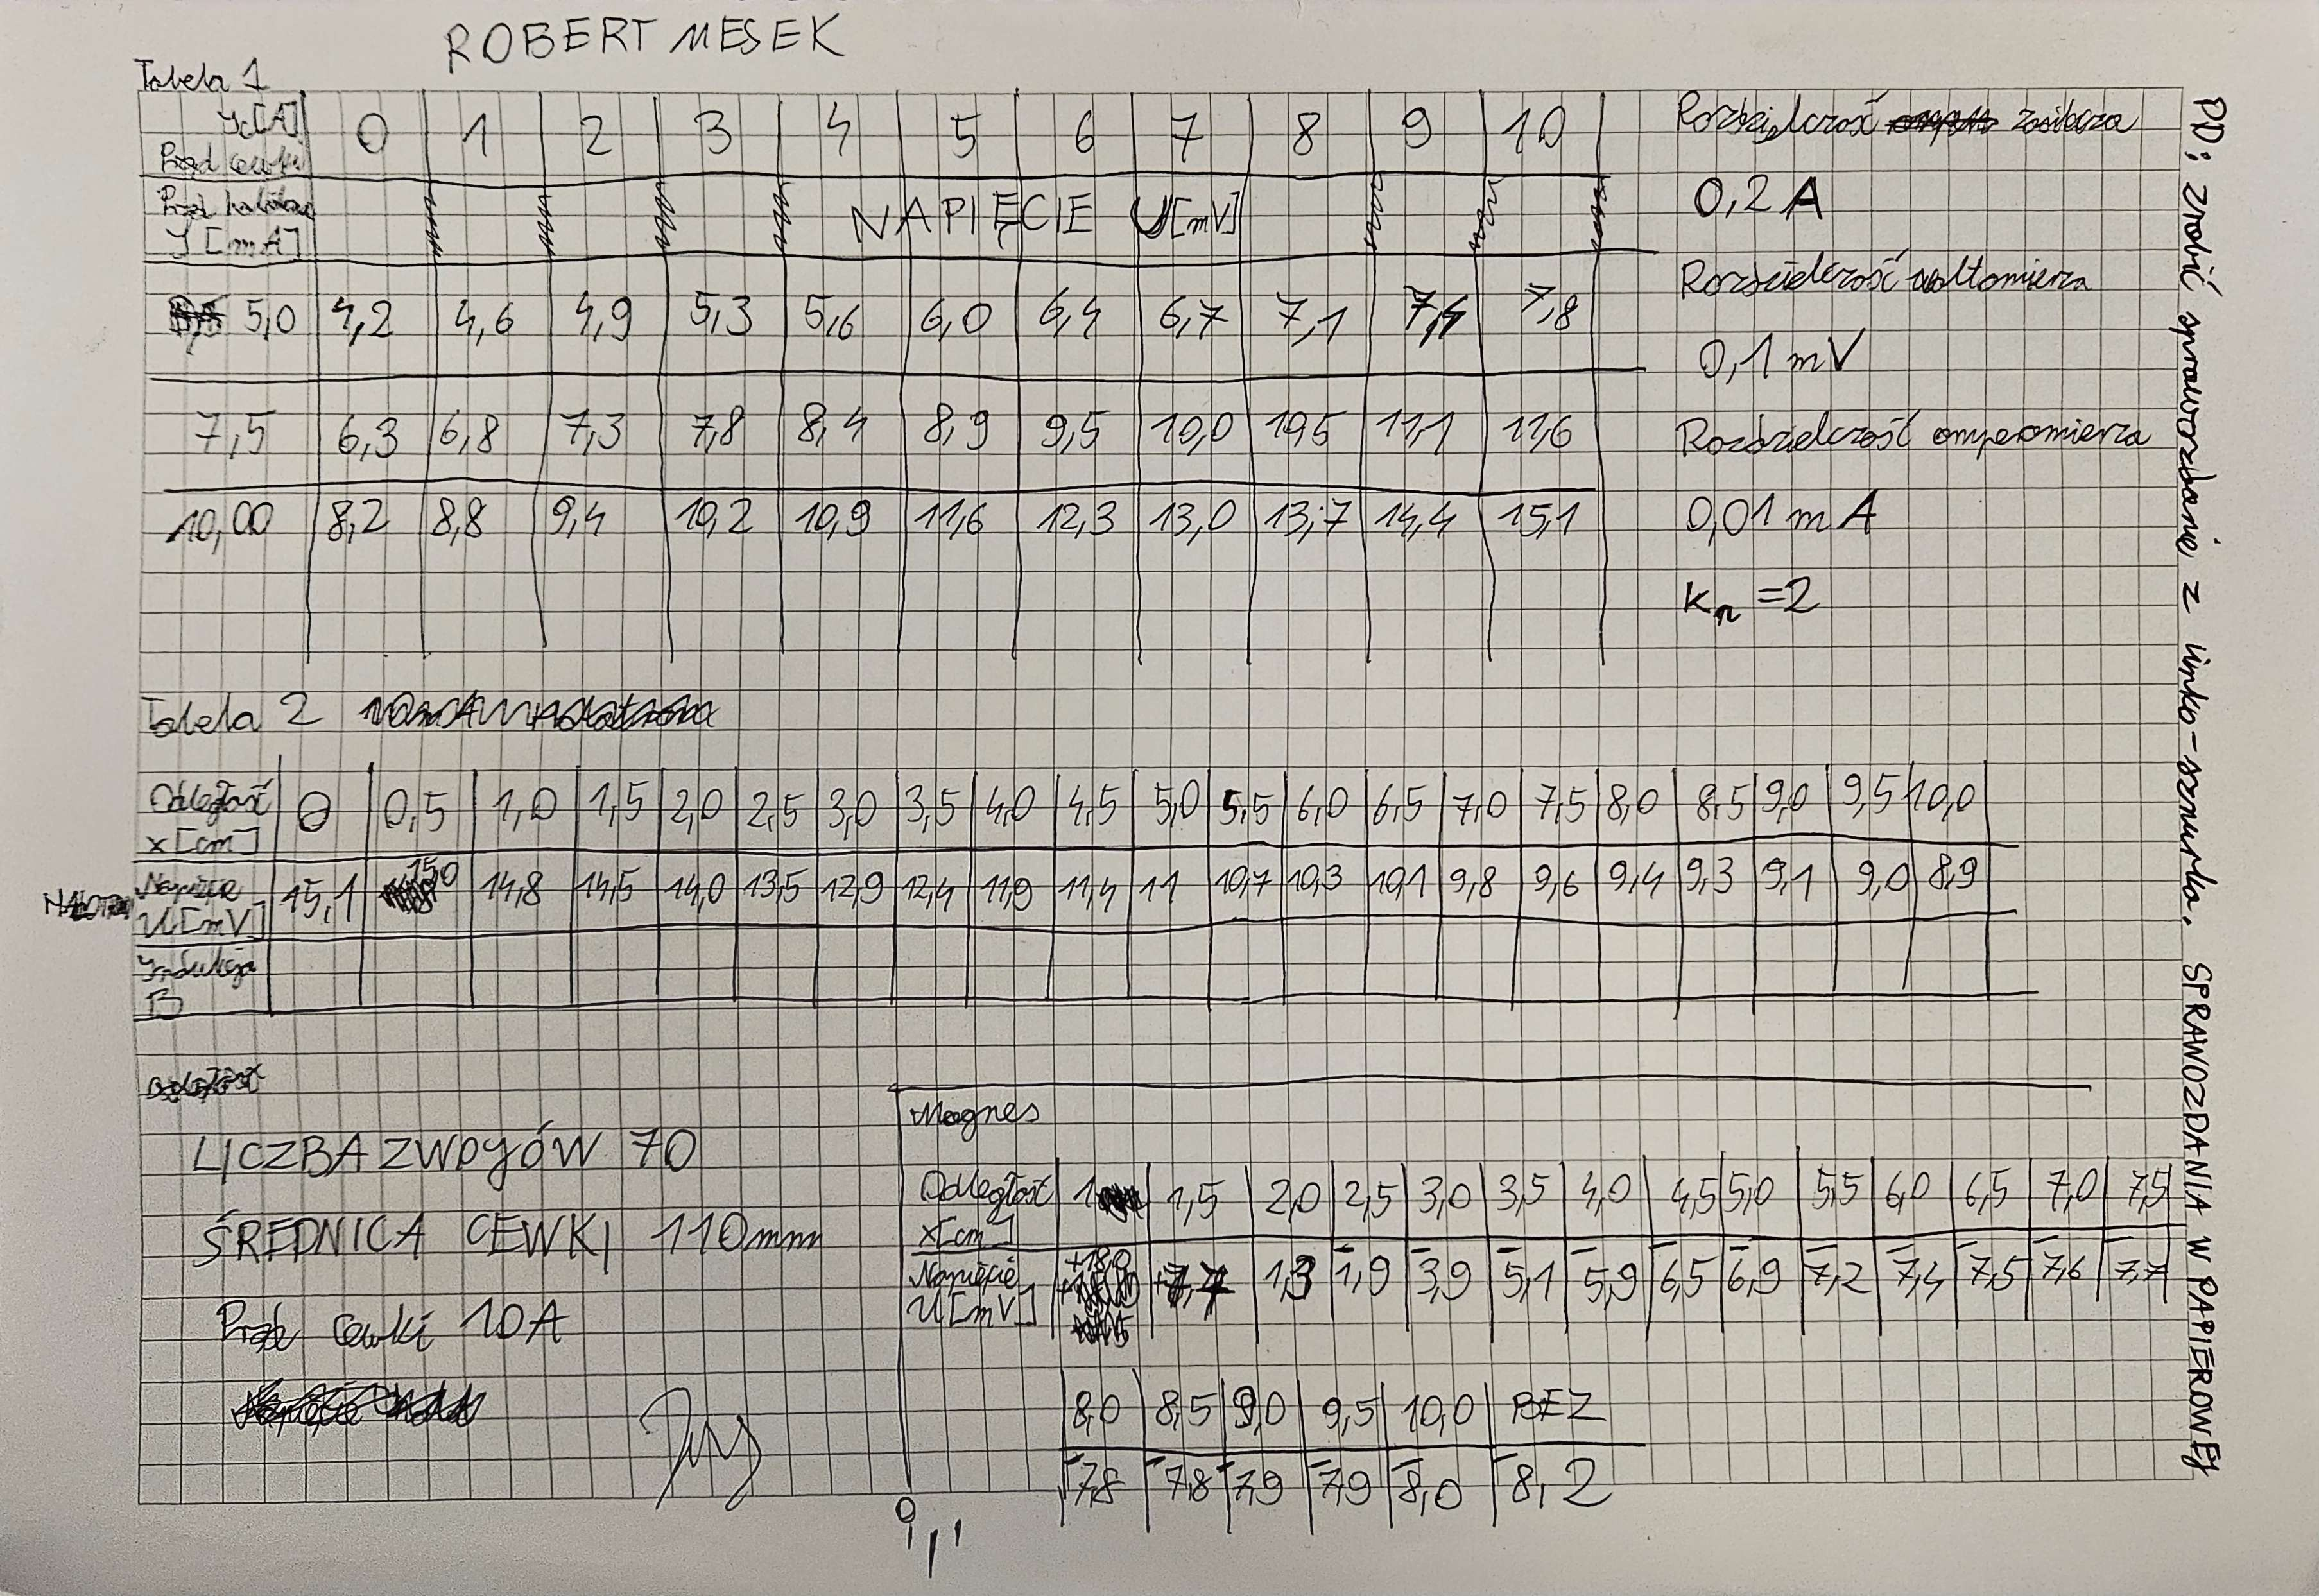
\includegraphics[width=1.5\linewidth, angle=270]{images/pomiary.jpg}
	\centering
\end{figure}
%\section*{Bibliografia}
% {\setlength{\parindent}{0pt}
%
% }

\end{document}
